% Created 2014-01-26 dom 13:51
\documentclass[a4paper,12pt]{report}
\usepackage{fancyhdr}
\usepackage{lastpage}
\usepackage{extramarks}
\usepackage[usenames,dvipsnames]{color}
\usepackage{graphicx}
\usepackage{courier}
\usepackage{lipsum}
\usepackage{wrapfig}
\usepackage{geometry}
\usepackage{alltt}
\usepackage{textcomp}
\usepackage{ifthen}
\usepackage{adjustbox}
\usepackage[table]{xcolor}
\usepackage{caption}
\usepackage{subcaption}
\usepackage{hyperref}
\usepackage{titlesec}

\topmargin=-0.45in
\evensidemargin=0in
\oddsidemargin=0in
\textwidth=6.5in
\textheight=9.0in
\headsep=0.25in
\linespread{1.1}
\pagestyle{fancy}
\lhead{\hmwkLeft}
\chead{\hmwkCenter}
\rhead{\hmwkRight}
\lfoot{\lastxmark}
\cfoot{}
\rfoot{Página\ \thepage\ de\ \protect\pageref{LastPage}}
\renewcommand\headrulewidth{0.4pt}
\renewcommand\footrulewidth{0.4pt}
\setlength\parindent{0pt}
\setlength{\headheight}{15pt}
\definecolor{darkgreen}{rgb}{0.0,0.25,0.08}
\definecolor{ligthgreen}{rgb}{0.0,0.50,0.08}
\definecolor{Negro}{HTML}{000000}
\definecolor{listinggray}{gray}{0.9}
\definecolor{lbcolor}{rgb}{0.9,0.9,0.9}
\definecolor{darkblue}{rgb}{0,0.08,0.45}
\definecolor{malva}{HTML}{D28FFF}
\definecolor{azulito}{HTML}{62CDF5}
\hypersetup{
    colorlinks,
    citecolor=darkgreen,
    filecolor=darkgreen,
    linkcolor=darkgreen,
    urlcolor=darkgreen
}
\geometry{a4paper,tmargin=20mm,bmargin=20mm,lmargin=20mm,rmargin=20mm}
\titleformat{\chapter}[display]{\normalfont\huge\sffamily\bfseries\filcenter}{\vspace*{-2cm}
\leavevmode\leaders\vrule height7pt width3pt depth0pt
\hfill\kern8pt\thechapter\kern8pt
\leaders\vrule height7pt width3pt depth0pt\hfill}{3pt}{\vspace*{-5pt}\hrule\vspace{6pt}}[\vspace{1pt}\hrule\vspace{1cm}]
\newcommand\Bheadfont{\fontsize{11pt}{\baselineskip}\selectfont}
\titleformat{\section}[hang]{\normalfont\sc\color{darkblue}\Bheadfont}{\thesection\hskip0.618em}{0em}{}
\titlespacing*{\section}{0pt}{15pt plus 2pt minus 2pt}{9pt plus 2pt minus 2pt}
\titleformat{\subsection}[hang]{\normalfont\sc\color{darkgreen}}{\thesubsection\hskip0.618em}{0em}{}
\titlespacing*{\subsection}{0pt}{8pt plus 2pt minus 2pt}{8pt plus 2pt minus 2pt}
\titleformat{\subsubsection}[hang]{\normalfont\it}{}{0.618em}{}
\titlespacing*{\subsubsection}{0pt}{8pt plus 2pt minus 2pt}{4pt plus 2pt minus 2pt}
\title{
\vspace{2in}
\textmd{\textbf{\hmwkClass:\ \hmwkTitle}}\\
\normalsize\vspace{0.1in}\small{\hmwkDueDate}\\
\vspace{0.1in}\large{\textit{\hmwkClassInstructor\ }}
\vspace{3in}
}
\author{\textbf{\hmwkAuthorName}}
\date{}


\usepackage{fontspec}
\usepackage{minted}
\usepackage{pifont}
\usepackage{pstricks, pst-node}
\usemintedstyle{perldoc}
\usepackage[section]{placeins}
\renewcommand{\contentsname}{ÍNDICE}
\renewcommand{\chaptername}{C}
\newcommand{\hmwkLeft}{}
\newcommand{\hmwkCenter}{\hmwkClass}
\newcommand{\hmwkRight}{\hmwkTitle}
\newcommand{\hmwkTitle}{Proyecto DDSI}
\newcommand{\hmwkTitleExtended}{Sistema de Información para el registro y control de alimentos y dietas}
\newcommand{\hmwkClass}{Desarrollo De Sistemas de Información}
\newcommand{\hmwkClassInstructor}{}
\newcommand{\hmwkAuthorName}{}
\setmonofont[Scale=0.7]{Monaco}
\setmonofont[Scale=0.9]{FreeMono}
\usepackage{paralist}
\usepackage{slashbox}
\let\itemize\compactitem
\let\itemize\compactitem
\renewcommand{\bibname}{Referencias}
\renewcommand{\figurename}{Figura}
\renewcommand{\tablename}{Tabla}
\date{\today}
\title{Memoria}
\hypersetup{
  pdfkeywords={},
  pdfsubject={},
  pdfcreator={Emacs 24.3.1 (Org mode 8.2.4)}}
\begin{document}

\title{
\begin{center}
\vspace*{-2.5cm}
\begin{figure}[htb]
\begin{center}
\includegraphics[width=4cm]{/home/dabuti/University/ugr.jpg}
\end{center}
\end{figure}
\end{center}
\Huge{\textbf{Universidad de Granada}}\\
\vspace{1cm}
\Huge{\textbf{Grado en Ingeniería Informática}}\\
\vspace{2cm}
\hrule{}
\vspace{0.3cm}
\textbf{\hmwkClass}\\
\vspace{0.3cm}
\hrule{}
\vspace{2cm}
\textbf{\hmwkTitle}\\
\vspace{1cm}
\textbf{\hmwkTitleExtended}\\
\vspace{1.5cm}
\textbf{\small{Iris García de Sebastián}}\\
\textbf{\small{David Santiago Carrión}}\\
\vspace{0.1cm}
}

\maketitle
\clearpage
\tableofcontents
\clearpage

\chapter{Descripción}
\label{sec-1}
Se pretende implementar un sistema para registrar las comidas que se
llevan a cabo a lo largo del día y gestionar los alimentos. Para
ello se almacenarán los ingredientes que componen cada receta y su
cantidad, además de información nutricional acerca de cada alimento
y el lugar y precio donde lo adquirimos.


\section{Registro de alimentos}
\label{sec-1-1}
Al introducir los productos adquiridos en un supermercado estos
deben agruparse en categorías con un nivel de abstracción
superior, considerados como ingredientes. Por ejemplo si el
usuario compra una botella de aceite  de oliva 'Jucaso' en el
supermercado 'Coviran' y otra botella de aceite de oliva 'Borges'
en el supermercado Mercadona, ambos producto deben almacenarse en
el sistema bajo el producto 'aceite de oliva'.

De este modo cada producto que empleemos en la elaboración de
nuestra alimentación diaria está descrito por:
\begin{itemize}
\item \textbf{nombre del producto}: una serie de caracteres.
\item \textbf{energía}: un número que indica las kilocalorías que aporta por
cada 100 gramos de producto.
\item \textbf{Descripción}: detalles y explicaciones acerca del alimento.
\end{itemize}

Los alimentos los podemos adquirir en distintos establecimientos,
lo cual nos lleva a guardar información relevante acerca de los
mismos como:
\begin{itemize}
\item \textbf{nombre del establecimiento}: una serie de caracteres.
\item \textbf{dirección}: caracteres alfanuméricos que nos ayudan a ubicar la tienda.
\item \textbf{teléfono}: caracteres numéricos.
\item \textbf{web}: dirección web del comercio.
\end{itemize}

Tanto los datos de los alimentos como los de los supermercados
podrán ser modificados.


Cada vez que se hace una compra se registra información de los
productos adquiridos:
\begin{itemize}
\item \textbf{producto}: el producto comprado.
\item \textbf{establecimiento}: donde lo hemos comprado.
\item \textbf{comprador}: el usuario que ha realizado la compra.
\item \textbf{cantidad}: número de unidades adquiridas del producto.
\item \textbf{precio}: número que indica el coste total.
\item \textbf{fecha}: cuando se realizó la adquisición.
\end{itemize}

$\backslash$\newpage

\section{Registro de dietas}
\label{sec-1-2}
Con todos los ingredientes adquirdos se pueden cocinar recetas. Las
recetas se describen y se almacena en el sistema teniendo en cuenta
los siguientes puntos:
\begin{itemize}
\item \textbf{nombre}: una serie de caracteres.
\item \textbf{personas}: número de comensales a los que puede abastecer.
\item \textbf{ingredientes}: un conjunto formado por los alimentos necesarios.
\item \textbf{cantidad}: indica la proporción de cada ingrediente.
\item \textbf{tiempo}: minutos que nos puede costar cocinarlo.
\item \textbf{valor nutricional}: número total de calorías que aporta la
receta.
\item \textbf{descripción}: documento que indica los pasos a seguir para
realizar el plato.
\end{itemize}

\vspace{0.2cm}
A partir de las diferentes recetas se pueden crear listas
personalizadas de las mismas, generando dietas. Las dietas son
creadas por los usuarios y les pertenecen a ellos exclusivamente. A
diferencia de las recetas estas no se comparten.

Se guardarán los siguientes puntos:
\begin{itemize}
\item \textbf{nombre de la dieta}: una serie de caracteres.
\item \textbf{recetas}: el conjunto de recetas asociado a la dieta.
\item \textbf{descripción}: información adicional sobre la dieta descrita.
\item \textbf{usuario}: identifica al propietario de la dieta.
\end{itemize}

\vspace{0.2cm}
Tanto las recetas como las dietas han de poder ser editadas,
eliminando y agregando ingredientes o recetas según el caso.

Dada una dieta en concreto, se listará la información general de la
misma junto con sus recetas asociadas, permitiendo al usuario
hacerse una idea de los platos que puede preparar.

Cada vez que alguien realiza una receta se registra quien cocinó la
comida, para llevar un control de la despensa:
\begin{itemize}
\item \textbf{Usuario}: quien la ha cocinado.
\item \textbf{Receta}: que receta se ha cocinado.
\item \textbf{Fecha}: cuando se ha realizado la comida.
\end{itemize}

\vspace{0.2cm}
Los usuarios podrán ver los platos que han realizado y se les
ofrecerá la opción de eliminar una comida registrada, para subsanar
posibles errores de registro.

$\backslash$\newpage

\section{Registro de usuarios}
\label{sec-1-3}
La base de usuarios estarán registrados, permitiéndoles realizar
dietas específicas, comidas, compras o recetas. Sus datos serían:
\begin{itemize}
\item \textbf{nombre}: una serie de caracteres.
\item \textbf{primer apellido}: caracteres alfabéticos.
\item \textbf{segundo apellido}:  una serie de caracteres.
\item \textbf{nick}: caracteres por los que quiere ser identificado.
\item \textbf{contraseña}: combinación necesaria para entrar al sistema.
\end{itemize}

\vspace{0.2cm}
Los usuarios anónimos tienen la opción de darse de alta en el
sistema proporcionando los datos previamente expuestos. A partir de
entonces podrán acceder a las distintas operaciones que ofrece el
sistema, así como editar o eliminar su perfil.


\section{Información y estadísticas}
\label{sec-1-4}
Los usuarios del sistema tienen acceso a información extraida de
las acciones que han ido llevando a cabo con el uso cotidiano del
sistema.

De este modo podrán acceder a una lista con todos los alimentos que
tienen disponibles actualmente en la despensa y a una lista de
recetas que pueden ser cocinadas en vista de los ingredientes con
los que cuenta y las dietas que ha creado.

Cuando un usuario crea una dieta y asocia los platos que desea,
podrá obtener el coste que le supondría adquirir los productos, en
los distintos supermercados, para ejecutar todos los platos de
dicha dieta.

Por último, el usuario deberá poder obtener su gasto medio en
euros, tanto el diario como desde el inicio del presente mes.
\chapter{Análisis de requisitos}
\label{sec-2}
\section{Requisitos de datos}
\label{sec-2-1}
\subsection{RD1-Datos nuevo producto}
\label{sec-2-1-1}
\begin{itemize}
\item \textbf{Nombre}: una cadena de hasta 20 caracteres no vacía.
\item \textbf{Calorías}: un número decimal positivo.
\item \textbf{Descripción}: una cadena de hasta 200 caracteres.
\end{itemize}

\subsection{RD2-Datos producto:}
\label{sec-2-1-2}
\begin{itemize}
\item \textbf{Identificador} de producto: un número entero.
\item \textbf{Nombre}: una cadena de hasta 20 caracteres no vacía.
\item \textbf{Calorías}: un número decimal positivo.
\item \textbf{Descripción}: una cadena de hasta 200 caracteres.
\end{itemize}
\subsection{RD3-Datos producto modificado:}
\label{sec-2-1-3}
\begin{itemize}
\item \textbf{Identificador} de producto: un número entero.
\item \textbf{Nombre}: una cadena de hasta 20 caracteres.
\item \textbf{Calorías}: un número decimal positivo.
\item \textbf{Descripción}: una cadena de hasta 200 caracteres.
\end{itemize}
\subsection{RD4-Identificador comprador:}
\label{sec-2-1-4}
\begin{itemize}
\item \textbf{Identificador} de usuario: un número entero.
\end{itemize}
\subsection{RD5-Lista de productos comprados:}
\label{sec-2-1-5}
\begin{itemize}
\item \textbf{Identificador} de producto: un número entero.
\item \textbf{Nombre}: una cadena de hasta 20 caracteres no vacía.
\item \textbf{Calorías}: un número decimal positivo.
\item \textbf{Descripción}: una cadena de hasta 200 caracteres.
\end{itemize}
\subsection{RD6-Datos nuevo super:}
\label{sec-2-1-6}
\begin{itemize}
\item \textbf{Nombre}:  una cadena de hasta 20 caracteres no vacía.
\item \textbf{Dirección}:  una cadena de hasta 30 caracteres no vacía.
\item \textbf{Teléfono}: una cadena de 9 caracteres numéricos.
\item \textbf{Página} web: una cadena de hasta 20 caracteres no vacía.
\end{itemize}
\subsection{RD7-Datos super:}
\label{sec-2-1-7}
\begin{itemize}
\item \textbf{Identificador} de super: un número entero.
\item \textbf{Nombre}:  una cadena de hasta 20 caracteres no vacía.
\item \textbf{Dirección}:  una cadena de hasta 30 caracteres.
\item \textbf{Teléfono}: una cadena de hasta 9 caracteres numéricos.
\item \textbf{Página web}: una cadena de hasta 20 caracteres.
\end{itemize}
\subsection{RD8-Datos super modificado:}
\label{sec-2-1-8}
\begin{itemize}
\item \textbf{Identificador de super}: un número entero.
\item \textbf{Nombre}:  una cadena de hasta 20 caracteres.
\item \textbf{Dirección}:  una cadena de hasta 30 caracteres.
\item \textbf{Teléfono}: una cadena de hasta 9 caracteres numéricos.
\item \textbf{Página web}: una cadena de hasta 20 caracteres.
\end{itemize}
\subsection{RD9-Datos nueva compra:}
\label{sec-2-1-9}
\begin{itemize}
\item \textbf{Identificador} de usuario: un número entero.
\end{itemize}
\subsection{RD10-Datos compra:}
\label{sec-2-1-10}
\begin{itemize}
\item \textbf{Identificador de compra}: un número entero.
\item \textbf{Identificador de usuario}: un número entero.
\item \textbf{Fecha}: tres conjuntos de enteros formados los dos primeros por conjuntos de dos cifras y el                 tercero por un conjunto de cuatro cifras, separados por barras ('/').
\end{itemize}
\subsection{RD11-Datos nueva línea de compra:}
\label{sec-2-1-11}
\begin{itemize}
\item \textbf{Identificador de compra}: un número entero.
\item \textbf{Identificador de producto}: un número entero.
\item \textbf{Identificador de super}: un número entero.
\item \textbf{Cantidad}: un número entero mayor que cero.
\item \textbf{Importe}: un número decimal mayor que cero.
\end{itemize}
\subsection{RD12-Datos línea de compra:}
\label{sec-2-1-12}
\begin{itemize}
\item \textbf{Identificador de compra}: un número entero.
\item \textbf{Identificador de producto}: un número entero.
\item \textbf{Identificador de super}: un número entero.
\item \textbf{Cantidad}: un número entero mayor que cero.
\item \textbf{Importe}: un número decimal mayor que cero.
\end{itemize}
\subsection{RD13-Datos línea de compra a eliminar:}
\label{sec-2-1-13}
\begin{itemize}
\item \textbf{Identificador de compra}: un número entero.
\item \textbf{Identificador de producto}: un número entero.
\item \textbf{Identificador de super}: un número entero.
\end{itemize}
\subsection{RD14-Datos nueva dieta:}
\label{sec-2-1-14}
\begin{itemize}
\item \textbf{Identificador de usuario}: un número entero.
\item \textbf{Nombre}: una cadena de hasta 20 caracteres no vacía.
\item \textbf{Descripción}: una cadena de hasta 200 caracteres.
\end{itemize}
\subsection{RD15-Datos dieta:}
\label{sec-2-1-15}
\begin{itemize}
\item \textbf{Identificador de dieta}: un número entero.
\item \textbf{Identificador de usuario}: un número entero.
\item \textbf{Nombre}: una cadena de hasta 20 caracteres no vacía.
\item \textbf{Descripción}: una cadena de hasta 200 caracteres.
\end{itemize}
\subsection{RD16-Datos nueva receta de dieta:}
\label{sec-2-1-16}
\begin{itemize}
\item \textbf{Identificador de dieta}: un número entero.
\item \textbf{Identificador de receta}: un número entero.
\end{itemize}
\subsection{RD17-Datos receta de dieta:}
\label{sec-2-1-17}
\begin{itemize}
\item \textbf{Identificador de dieta}: un número entero.
\item \textbf{Identificador de receta}: un número entero.
\end{itemize}
\subsection{RD18-Datos receta de dieta a eliminar:}
\label{sec-2-1-18}
\begin{itemize}
\item \textbf{Identificador de dieta}: un número entero.
\item \textbf{Identificador de receta}: un número entero.
\end{itemize}
\subsection{RD19-Datos nueva receta:}
\label{sec-2-1-19}
\begin{itemize}
\item \textbf{Nombre}: una cadena de hasta 20 caracteres no vacía.
\item \textbf{Personas}: un número entero.
\item \textbf{Tiempo}: un número entero.
\item \textbf{Descripción}: una cadena de hasta 200 caracteres.
\end{itemize}
\subsection{RD20-Datos receta:}
\label{sec-2-1-20}
\begin{itemize}
\item \textbf{Identificador de receta}: un número entero.
\item \textbf{Nombre}: una cadena de hasta 20 caracteres no vacía.
\item \textbf{Personas}: un número entero mayor que cero.
\item \textbf{Tiempo}: un número entero mayor que cero.
\item \textbf{Descripción}: una cadena de hasta 200 caracteres.
\end{itemize}
\subsection{RD21-Datos nuevo producto de receta:}
\label{sec-2-1-21}
\begin{itemize}
\item \textbf{Identificador de producto}: un número entero.
\item \textbf{Identificador de receta}: un número entero.
\item \textbf{Cantidad}: un número entero.
\end{itemize}
\subsection{RD22-Datos producto de receta:}
\label{sec-2-1-22}
\begin{itemize}
\item \textbf{Identificador de producto}: un número entero.
\item \textbf{Identificador de receta}: un número entero.
\item \textbf{Cantidad}: un número entero.
\end{itemize}
\subsection{RD23-Datos producto de receta a eliminar:}
\label{sec-2-1-23}
\begin{itemize}
\item \textbf{Identificador de producto}: un número entero.
\item \textbf{Identificador de receta}: un número entero.
\end{itemize}
\subsection{RD24-Datos receta modificada:}
\label{sec-2-1-24}
\begin{itemize}
\item \textbf{Identificador de receta}: un número entero.
\item \textbf{Nombre}: una cadena de hasta 20 caracteres.
\item \textbf{Personas}: un número entero.
\item \textbf{Tiempo}: un número entero.
\item \textbf{Descripción}: una cadena de hasta 200 caracteres.
\end{itemize}
\subsection{RD25-Datos nuevo usuario:}
\label{sec-2-1-25}
\begin{itemize}
\item \textbf{Nombre}: una cadena de hasta 20 caracteres no vacía.
\item \textbf{Primer apellido}: una cadena de hasta 20 caracteres.
\item \textbf{Segundo apellido}: una cadena de hasta 20 caracteres.
\item \textbf{Nombre de usuario}: una cadena de hasta 20 caracteres.
\item \textbf{Contraseña}: una cadena alfanumérica de hasta 20 elementos.
\end{itemize}
\subsection{RD26-Datos usuario:}
\label{sec-2-1-26}
\begin{itemize}
\item \textbf{Identificador de usuario}: un número entero.
\item \textbf{Nombre}: una cadena de hasta 20 caracteres no vacía.
\item \textbf{Primer apellido}: una cadena de hasta 20 caracteres.
\item \textbf{Segundo apellido}: una cadena de hasta 20 caracteres.
\item \textbf{Nombre de usuario}: una cadena de hasta 20 caracteres.
\item \textbf{Contraseña}: una cadena alfanumérica de hasta 20 elementos.
\end{itemize}
\subsection{RD27-Datos usuario modificado:}
\label{sec-2-1-27}
\begin{itemize}
\item \textbf{Identificador de usuario}: un número entero.
\item \textbf{Nombre}: una cadena de hasta 20 caracteres no vacía.
\item \textbf{Primer apellido}: una cadena de hasta 20 caracteres.
\item \textbf{Segundo apellido}: una cadena de hasta 20 caracteres.
\item \textbf{Contraseña}: una cadena alfanumérica de hasta 20 elementos.
\end{itemize}

\subsection{RD28-Datos usuario a eliminar:}
\label{sec-2-1-28}
\begin{itemize}
\item \textbf{Identificador de usuario}: un número entero.
\end{itemize}
\subsection{RD29-Datos nueva comida:}
\label{sec-2-1-29}
\begin{itemize}
\item \textbf{Identificador de usuario}: un número entero.
\item \textbf{Identificador de receta}: un número entero.
\item \textbf{Fecha}: tres conjuntos de enteros formados los dos primeros por conjuntos de dos cifras y el                 tercero por un conjunto de cuatro cifras, separados por barras ('/').
\end{itemize}
\subsection{RD30-Datos comida:}
\label{sec-2-1-30}
\begin{itemize}
\item \textbf{Identificador de usuario}: un número entero.
\item \textbf{Identificador de receta}: un número entero.
\item \textbf{Fecha}: tres conjuntos de enteros formados los dos primeros por conjuntos de dos cifras y el                 tercero por un conjunto de cuatro cifras, separados por barras ('/').
\end{itemize}
\subsection{RD31-Identificador propietario de stock:}
\label{sec-2-1-31}
\begin{itemize}
\item \textbf{Identificador de usuario}: un número entero.
\end{itemize}
\subsection{RD32-Lista de stock:}
\label{sec-2-1-32}
\begin{itemize}
\item \textbf{Identificador de producto}: un número entero.
\item \textbf{Nombre}: una cadena de hasta 20 caracteres no vacía.
\item \textbf{Calorías}: un número decimal positivo.
\item \textbf{Descripción}: una cadena de hasta 200 caracteres.
\item \textbf{Cantidad}: un número entero mayor que cero.
\end{itemize}
\subsection{RD33-Identificador usuario para gasto diario:}
\label{sec-2-1-33}
\begin{itemize}
\item \textbf{Identificador de usuario}: un número entero.
\end{itemize}
\subsection{RD34-Valor de gasto diario:}
\label{sec-2-1-34}
\begin{itemize}
\item \textbf{Gasto}: un número decimal.
\end{itemize}
\subsection{RD35-Identificador usuario para gasto mensual:}
\label{sec-2-1-35}
\begin{itemize}
\item \textbf{Identificador de usuario}: un número entero.
\end{itemize}
\subsection{RD36-Valor de gasto mensual:}
\label{sec-2-1-36}
\begin{itemize}
\item \textbf{Gasto}: un número decimal.
\end{itemize}
\subsection{RD37-Usuario que consulta recetas disponibles:}
\label{sec-2-1-37}
\begin{itemize}
\item \textbf{Identificador de usuario}: un número entero.
\end{itemize}
\subsection{RD38-Lista recetas disponibles:}
\label{sec-2-1-38}
\begin{itemize}
\item \textbf{Identificador de receta}: un número entero.
\item \textbf{Nombre}: una cadena de hasta 20 caracteres no vacía.
\item \textbf{Personas}: un número entero mayor que cero.
\item \textbf{Tiempo}: un número entero mayor que cero.
\item \textbf{Descripción}: una cadena de hasta 200 caracteres.
\end{itemize}
\subsection{RD39-Identificador de dieta a consultar:}
\label{sec-2-1-39}
\begin{itemize}
\item \textbf{Identificador de dieta}: un número entero.
\end{itemize}
\subsection{RD40-Coste por super:}
\label{sec-2-1-40}
\begin{itemize}
\item \textbf{Identificador de super}: un número entero.
\item \textbf{Nombre}:  una cadena de hasta 20 caracteres no vacía.
\item \textbf{Dirección}:  una cadena de hasta 30 caracteres.
\item \textbf{Teléfono}: una cadena de hasta 9 caracteres numéricos.
\item \textbf{Página web}: una cadena de hasta 20 caracteres.
\item \textbf{Gasto}: un número decimal.
\end{itemize}
\subsection{RD41-Datos de identificación:}
\label{sec-2-1-41}
\begin{itemize}
\item \textbf{Nombre}: una cadena de hasta 20 caracteres no vacía.
\item \textbf{Contraseña}: una cadena alfanumérica de hasta 20 elementos no vacía.
\end{itemize}
\subsection{RD42-Identificador creador de dieta:}
\label{sec-2-1-42}
\begin{itemize}
\item \textbf{Identificador de usuario}: un número entero.
\end{itemize}
\subsection{RD43-Identificador usuario:}
\label{sec-2-1-43}
\begin{itemize}
\item \textbf{Identificador de usuario}: un número entero.
\end{itemize}

\subsection{RD44-Lista de recetas de dieta:}
\label{sec-2-1-44}
\begin{itemize}
\item \textbf{Identificador de receta}: un número entero.
\item \textbf{Nombre}: una cadena de hasta 20 caracteres.
\item \textbf{Personas}: un número entero.
\item \textbf{Tiempo}: un número entero.
\item \textbf{Descripción}: una cadena de hasta 200 caracteres.
\end{itemize}
\subsection{RD45-Identificador creador de dietas:}
\label{sec-2-1-45}
\begin{itemize}
\item \textbf{Identificador de usuario}: un número entero.
\end{itemize}
\subsection{RD46-Lista de dietas:}
\label{sec-2-1-46}
\begin{itemize}
\item \textbf{Identificador de dieta}: un número entero.
\item \textbf{Nombre}: una cadena de hasta 20 caracteres no vacía.
\item \textbf{Descripción}: una cadena de hasta 200 caracteres.
\end{itemize}
\subsection{RD47-Identificador consultor de recetas:}
\label{sec-2-1-47}
\begin{itemize}
\item \textbf{Identificador de usuario}: un número entero.
\end{itemize}
\subsection{RD48-Lista de recetas:}
\label{sec-2-1-48}
\begin{itemize}
\item \textbf{Identificador de receta}: un número entero.
\item \textbf{Nombre}: una cadena de hasta 20 caracteres.
\item \textbf{Personas}: un número entero.
\item \textbf{Tiempo}: un número entero.
\item \textbf{Descripción}: una cadena de hasta 200 caracteres.
\end{itemize}
\subsection{RD49-Identificador usuario propio:}
\label{sec-2-1-49}
\begin{itemize}
\item \textbf{Identificador de usuario}: un número entero.
\end{itemize}
\subsection{RD50-Datos usuario propio:}
\label{sec-2-1-50}
\begin{itemize}
\item \textbf{Nombre}: una cadena de hasta 20 caracteres.
\item \textbf{Primer apellido}: una cadena de hasta 20 caracteres.
\item \textbf{Segundo apellido}: una cadena de hasta 20 caracteres.
\item \textbf{Nombre de usuario}: una cadena de hasta 20 caracteres.
\item \textbf{Contraseña}: una cadena alfanumérica de hasta 20 elementos.
\end{itemize}
\subsection{RD51-Identificador cocinero:}
\label{sec-2-1-51}
\begin{itemize}
\item \textbf{Identificador de usuario}: un número entero.
\end{itemize}
\subsection{RD52-Lista de comidas:}
\label{sec-2-1-52}
\begin{itemize}
\item \textbf{Identificador de usuario}: un número entero.
\item \textbf{Identificador de receta}: un número entero.
\item \textbf{Fecha}: tres conjuntos de enteros formados los dos primeros por
conjuntos de dos cifras y el tercero por un conjunto de cuatro
cifras, separados por barras ('/').
\end{itemize}
\subsection{RD53-Datos comida a eliminar:}
\label{sec-2-1-53}
\begin{itemize}
\item \textbf{Identificador de usuario}: un número entero.
\item \textbf{Identificador de receta}: un número entero.
\item \textbf{Fecha}: tres conjuntos de enteros formados los dos primeros por
conjuntos de dos cifras y el tercero por un conjunto de cuatro
cifras, separados por barras ('/').
\end{itemize}
\section{Requisitos funcionales}
\label{sec-2-2}
\subsection{\textbf{RF1-Alta de un producto}: registra un producto en el sistema a partir de los datos de un producto proporcionados por un usuario.}
\label{sec-2-2-1}

\subsection{\textbf{RF2-Modificar un producto}: modifica los datos de un producto almacenado en el sistema por los proporcionados por el usuario.}
\label{sec-2-2-2}

\subsection{\textbf{RF3-Listar productos comprados}: devuelve los productos comprados por el usuario cuyo código se ha pasado como parámetro.}
\label{sec-2-2-3}

\subsection{\textbf{RF4-Registrar un super}: añade un nuevo supermercado al sistema con la información facilitada por el usuario.}
\label{sec-2-2-4}

\subsection{\textbf{RF5-Modificar un super}: altera la información de un supermercado registrado en el sistema por los nuevos datos suministrados.}
\label{sec-2-2-5}

\subsection{\textbf{RF6-Nueva compra}: almacena una compra nueva en el sistema con la fecha actual y el identificador del usuario que la ha iniciado.}
\label{sec-2-2-6}

\subsection{\textbf{RF7-Añadir producto a compra}: incluye una cantidad determinada de artículos identificados por los datos proporcionados por el usuario y su importe en euros.}
\label{sec-2-2-7}

\subsection{\textbf{RF8-Eliminar producto de compra}: borra de una compra el producto adquirido en un supermercado  por el usuario.}
\label{sec-2-2-8}

\subsection{\textbf{RF9-Añadir nueva dieta}: agrega una nueva dieta a las almacenadas en el sistema a partir de los datos dados por el usuario.}
\label{sec-2-2-9}

\subsection{\textbf{RF10-Añadir receta a dieta}: incluye una receta en una dieta, ambas identificadas por los datos proporcionador por el usuario.}
\label{sec-2-2-10}

\subsection{\textbf{RF11-Eliminar receta de dieta}: borra una receta de una dieta determinada, según los datos proporcionados por el usuario.}
\label{sec-2-2-11}

\subsection{\textbf{RF12-Añadir nueva receta}: registra una receta en el sistema partiendo de los datos de una receta proporcionados por un usuario.}
\label{sec-2-2-12}

\subsection{\textbf{RF13-Añadir producto a receta}: registra un ingrediente, junto con su cantidad, en una receta almacenada en el sistema, a partir de los datos introducidos por el usuario.}
\label{sec-2-2-13}

\subsection{\textbf{RF14-Eliminar producto de receta}: elimina el producto identificado por el usuario de la receta proporcionada por el mismo.}
\label{sec-2-2-14}

\subsection{\textbf{RF15-Modificar una receta}: altera la información de una receta registrada en el sistema por los nuevos datos que el usuario proporcione.}
\label{sec-2-2-15}

\subsection{\textbf{RF16-Dar de alta un usuario}: registra un usuario nuevo en el sistema a partir de la información proporcionada por un usuario anónimo.}
\label{sec-2-2-16}

\subsection{\textbf{RF17-Modificar un usuario}: modifica los datos de un usuario registrado en el sistema e identificado por los nuevos valores suministrados.}
\label{sec-2-2-17}

\subsection{\textbf{RF18-Elimina un usuario}: suprime los datos de un usuario registrado en el sistema e identificado por los nuevos valores suministrados.}
\label{sec-2-2-18}

\subsection{\textbf{RF19-Hacer comida}: registra la elaboración de una receta llevada a cabo por un usuario del sistema en la fecha actual.}
\label{sec-2-2-19}

\subsection{\textbf{RF20-Listar stock}: muestra la cantidad de productos disponibles para un usuario.}
\label{sec-2-2-20}

\subsection{\textbf{RF21-Calcular gasto diario}: devuelve el promedio de euros que gasta el usuario cada día en comidas.}
\label{sec-2-2-21}

\subsection{\textbf{RF22-Calcular gasto mensual}: retorna la cantidad de euros que el usuario ha gastado este mes entre las comidas realizadas.}
\label{sec-2-2-22}

\subsection{\textbf{RF23-Mostrar recetas disponibles}: devuelve una lista con todas las recetas que, según los ingredientes disponibles y las dietas que sigue, se pueden cocinar.}
\label{sec-2-2-23}

\subsection{\textbf{RF24-Calcular precio de una dieta}: devuelve el coste de llevar a cabo cada receta de una dieta para cada supermercado.}
\label{sec-2-2-24}

\subsection{\textbf{RF25-Identificar usuario}: comprueba si los datos proporcionados por el usuarios anónimo coinciden con los de algún usuario registrado en el sistema y devuelve su clave.}
\label{sec-2-2-25}

\subsection{\textbf{RF26-Listar dieta completa}: muestra toda la información de las recetas asociadas a una dieta.}
\label{sec-2-2-26}

\subsection{\textbf{RF27-Listar dietas}: recoge del sistema todas las dietas asociadas al usuario y los devuelve en una lista.}
\label{sec-2-2-27}

\subsection{\textbf{RF28-Listar recetas}: devuelve una lista con todas las recetas del sistema, tanto las que pertenecen a alguna de nuestras dietas como las que no.}
\label{sec-2-2-28}

\subsection{\textbf{RF29-Mostrar datos usuario}: muestra los campos registrados asociados al identificador de usuario.}
\label{sec-2-2-29}

\subsection{\textbf{RF30-Listar comidas}: lista todos los platos que ha llevado a cabo el usuario del sistema.}
\label{sec-2-2-30}

\subsection{\textbf{RF31-Eliminar comida}: borra una comida registrada a partir de la receta y el identificador de usuario registrado.}
\label{sec-2-2-31}

\subsection{\textbf{Validación cruzada de requisitos}}
\label{sec-2-2-32}
\begin{figure}[!htp]
\centering
\includegraphics[width=0.9\linewidth]{./refinamientos/tablaRF1.png}
\caption{Requisitos funcionales}
\label{fig:Requisitos funcionales}
\medskip
\footnotesize
{}
\end{figure}

\begin{figure}[!htp]
\centering
\includegraphics[width=0.9\linewidth]{./refinamientos/tablaRF2.png}
\caption{Requisitos funcionales}
\label{fig:Requisitos funcionales}
\medskip
\footnotesize
{}
\end{figure}

\section{Restricciones semánticas}
\label{sec-2-3}
\subsection{RS1-No se pueden registrar usuarios con username repetidos.}
\label{sec-2-3-1}
\subsection{RS2-Todas las dietas deben estar asociadas a un usuario registrado.}
\label{sec-2-3-2}
\chapter{Esquema caja negra}
\label{sec-3}
\begin{figure}[!htp]
\centering
\includegraphics[width=0.9\linewidth]{./refinamientos/cajanegra.png}
\caption{Caja Negra}
\label{fig:Caja Negra}
\medskip
\footnotesize
{}
\end{figure}
\chapter{Refinamiento 0}
\label{sec-4}
\section{DFD 0 (Esquema Armazón)}
\label{sec-4-1}
\begin{figure}[!htp]
\centering
\includegraphics[width=0.9\linewidth]{./refinamientos/dfd0.png}
\caption{Esquema armazón}
\label{fig:Esquema armazón}
\medskip
\footnotesize
{}
\end{figure}
\section{Esquema externo 0}
\label{sec-4-2}
\begin{figure}[!htp]
\centering
\includegraphics[width=0.9\linewidth]{./refinamientos/externo0.png}
\caption{Externo 0}
\label{fig:Externo 0}
\medskip
\footnotesize
{}
\end{figure}
\section{Entidad Relación 0}
\label{sec-4-3}
\begin{figure}[!htp]
\centering
\includegraphics[width=0.6\linewidth]{./refinamientos/er0.png}
\caption{Entidad relación 0}
\label{fig:Entidad relación 0}
\medskip
\footnotesize
{}
\end{figure}
\chapter{Refinamiento 1}
\label{sec-5}
\section{DFD 1}
\label{sec-5-1}
\begin{figure}[!htp]
\centering
\includegraphics[width=0.9\linewidth]{./refinamientos/dfd1.png}
\caption{Diagrama de flujo de datos 1}
\label{fig:Diagrama de flujo de datos 1}
\medskip
\footnotesize
{}
\end{figure}
\section{Esquema externo 1}
\label{sec-5-2}
\begin{figure}[!htp]
\centering
\includegraphics[width=0.9\linewidth]{./refinamientos/externo1.png}
\caption{Externo 1}
\label{fig:Externo 1}
\medskip
\footnotesize
{}
\end{figure}
\section{Entidad Relación 1}
\label{sec-5-3}
\begin{figure}[!htp]
\centering
\includegraphics[width=0.7\linewidth]{./refinamientos/er1.png}
\caption{Entidad relación 1}
\label{fig:Entidad relación 1}
\medskip
\footnotesize
{}
\end{figure}
\chapter{Refinamiento 2}
\label{sec-6}
\section{DFD 2 (Esquema Armazón)}
\label{sec-6-1}
\begin{figure}[!htp]
\centering
\includegraphics[width=0.95\linewidth]{./refinamientos/dfd2.png}
\caption{Diagrama de flujo de datos 2}
\label{fig:Diagrama de flujo de datos 2}
\medskip
\footnotesize
{}
\end{figure}
\section{Esquema externo 2}
\label{sec-6-2}
\begin{figure}[!htp]
\centering
\includegraphics[width=0.9\linewidth]{./refinamientos/externo21.png}
\caption{Externo 2.1}
\label{fig:Externo 2.1}
\medskip
\footnotesize
{}
\end{figure}

\begin{figure}[!htp]
\centering
\includegraphics[width=0.9\linewidth]{./refinamientos/externo22.png}
\caption{Externo 2.2}
\label{fig:Externo 2.2}
\medskip
\footnotesize
{}
\end{figure}
\section{Entidad Relación 2}
\label{sec-6-3}
\begin{figure}[!htp]
\centering
\includegraphics[width=0.8\linewidth]{./refinamientos/er2.png}
\caption{Entidad relación 2}
\label{fig:Entidad relación 2}
\medskip
\footnotesize
{}
\end{figure}
\section{Entidad Relación final (atributos)}
\label{sec-6-4}
\begin{figure}[!htp]
\centering
\includegraphics[width=0.9\linewidth]{./refinamientos/erfinal.png}
\caption{Entidad relación final}
\label{fig:Entidad relación final}
\medskip
\footnotesize
{}
\end{figure}
\chapter{Esquemas de Operación y Navegación}
\label{sec-7}
\section{Proceso: Gestión Compras}
\label{sec-7-1}
\subsection{Lista de operaciones:}
\label{sec-7-1-1}
\begin{enumerate}
\item Listar el nombre, las calorías, la descripción, la cantidad, el precio de los productos, el nombre del supermercado y la fecha de las compras realizadas por un usuario a partir de su IDUsuario.
\begin{itemize}
\item Esquema de operación:
\begin{figure}[!htp]
\centering
\includegraphics[width=0.9\linewidth]{./operaciones/img/Compras/01_ope.png}
\caption{Esquema Operación - 01}
\label{fig:ope01}
\medskip
\footnotesize
{}
\end{figure}
\item Esquema de navegación:
\begin{figure}[!htp]
\centering
\includegraphics[width=0.9\linewidth]{./operaciones/img/Compras/01_nav.png}
\caption{Esquema Navegación - 01}
\label{fig:nave01}
\medskip
\footnotesize
{}
\end{figure}
\end{itemize}

\item Insertar una nueva compra.
NOTA: se inserta como Fecha un valor igual a la fecha actual de sistema.
\begin{itemize}
\item Esquema de operación:
\begin{figure}[!htp]
\centering
\includegraphics[width=0.9\linewidth]{./operaciones/img/Compras/02_ope.png}
\caption{Esquema Operación - 02}
\label{fig:ope02}
\medskip
\footnotesize
{}
\end{figure}
\item Esquema de navegación:
\begin{figure}[!htp]
\centering
\includegraphics[width=0.9\linewidth]{./operaciones/img/Compras/02_nav.png}
\caption{Esquema Navegación - 02}
\label{fig:nave02}
\medskip
\footnotesize
{}
\end{figure}
\end{itemize}

\item Asociar una comprar a partir del IDUsuario del usuario y el IDCompra de la compra.
\begin{itemize}
\item Esquema de operación:
\end{itemize}
\begin{figure}[!htp]
\centering
\includegraphics[width=0.9\linewidth]{./operaciones/img/Compras/03_ope.png}
\caption{Esquema Operación - 03}
\label{fig:ope03}
\medskip
\footnotesize
{}
\end{figure}
\begin{itemize}
\item Esquema de navegación:
\begin{figure}[!htp]
\centering
\includegraphics[width=0.9\linewidth]{./operaciones/img/Compras/03_nav.png}
\caption{Esquema Navegación - 03}
\label{fig:nave03}
\medskip
\footnotesize
{}
\end{figure}
\end{itemize}

\item Insertar una nueva línea de compra a partir del IDCompra, IDProducto
IDSuper, cantidad y precio.
\begin{itemize}
\item Esquema de operación:
\end{itemize}
\begin{figure}[!htp]
\centering
\includegraphics[width=0.9\linewidth]{./operaciones/img/Compras/04_ope.png}
\caption{Esquema Operación - 04}
\label{fig:ope04}
\medskip
\footnotesize
{}
\end{figure}
\begin{itemize}
\item Esquema de navegación:
\begin{figure}[!htp]
\centering
\includegraphics[width=0.9\linewidth]{./operaciones/img/Compras/04_nav.png}
\caption{Esquema Navegación - 04}
\label{fig:nave04}
\medskip
\footnotesize
{}
\end{figure}
\end{itemize}

\item Eliminar una línea de compra a partir del IDCompra, IDProducto e IDSuper.
\begin{itemize}
\item Esquema de operación:
\end{itemize}
\begin{figure}[!htp]
\centering
\includegraphics[width=0.9\linewidth]{./operaciones/img/Compras/05_ope.png}
\caption{Esquema Operación - 05}
\label{fig:ope05}
\medskip
\footnotesize
{}
\end{figure}
\begin{itemize}
\item Esquema de navegación:
\begin{figure}[!htp]
\centering
\includegraphics[width=0.9\linewidth]{./operaciones/img/Compras/05_nav.png}
\caption{Esquema Navegación - 05}
\label{fig:nave05}
\medskip
\footnotesize
{}
\end{figure}
\end{itemize}
\end{enumerate}
\section{Proceso: Gestión Productos}
\label{sec-7-2}
\subsection{Lista de operaciones}
\label{sec-7-2-1}
\begin{enumerate}
\item Insertar un producto a partir del nombre, descripción y
calorías.
\begin{itemize}
\item Esquema de operación:
\begin{figure}[!htp]
\centering
\includegraphics[width=0.9\linewidth]{./operaciones/img/Productos/01_ope.png}
\caption{Esquema Operación - 01}
\label{fig:ope01}
\medskip
\footnotesize
{}
\end{figure}
\item Esquema de navegación:
\begin{figure}[!htp]
\centering
\includegraphics[width=0.9\linewidth]{./operaciones/img/Productos/01_nav.png}
\caption{Esquema Navegación - 01}
\label{fig:nave01}
\medskip
\footnotesize
{}
\end{figure}
\end{itemize}

\item Modificar un producto a partir del IDProducto, nombre,
descripción y calorías.
\begin{itemize}
\item Esquema de operación:
\begin{figure}[!htp]
\centering
\includegraphics[width=0.9\linewidth]{./operaciones/img/Productos/02_ope.png}
\caption{Esquema Operación - 02}
\label{fig:ope02}
\medskip
\footnotesize
{}
\end{figure}
\item Esquema de navegación:
\begin{figure}[!htp]
\centering
\includegraphics[width=0.9\linewidth]{./operaciones/img/Productos/02_nav.png}
\caption{Esquema Navegación - 02}
\label{fig:nave02}
\medskip
\footnotesize
{}
\end{figure}
\end{itemize}

\item Asociar un producto a un super a partir del IDProducto y el IDSuper.
\begin{itemize}
\item Esquema de operación:
\begin{figure}[!htp]
\centering
\includegraphics[width=0.9\linewidth]{./operaciones/img/Productos/03_ope.png}
\caption{Esquema Operación - 03}
\label{fig:ope03}
\medskip
\footnotesize
{}
\end{figure}
\item Esquema de navegación:
\begin{figure}[!htp]
\centering
\includegraphics[width=0.9\linewidth]{./operaciones/img/Productos/03_nav.png}
\caption{Esquema Navegación - 03}
\label{fig:nave02}
\medskip
\footnotesize
{}
\end{figure}
\end{itemize}
\end{enumerate}
\section{Proceso: Gestión Supermercados}
\label{sec-7-3}
\subsection{Lista de operaciones}
\label{sec-7-3-1}
\begin{enumerate}
\item Insertar un supermercado a partir del nombre, dirección,
teléfono y página web.
\begin{itemize}
\item Esquema de operación:
\begin{figure}[!htp]
\centering
\includegraphics[width=0.9\linewidth]{./operaciones/img/Super/01_ope.png}
\caption{Esquema Operación - 01}
\label{fig:ope01}
\medskip
\footnotesize
{}
\end{figure}
\item Esquema de navegación:
\begin{figure}[!htp]
\centering
\includegraphics[width=0.9\linewidth]{./operaciones/img/Super/01_nav.png}
\caption{Esquema Navegación - 01}
\label{fig:nave01}
\medskip
\footnotesize
{}
\end{figure}
\end{itemize}

\item Modificar nombre, dirección, teléfono y página web de un
supermercado a partir del IDSuper.
\begin{itemize}
\item Esquema de operación:
\begin{figure}[!htp]
\centering
\includegraphics[width=0.9\linewidth]{./operaciones/img/Super/02_ope.png}
\caption{Esquema Operación - 02}
\label{fig:ope02}
\medskip
\footnotesize
{}
\end{figure}
\item Esquema de navegación:
\begin{figure}[!htp]
\centering
\includegraphics[width=0.9\linewidth]{./operaciones/img/Super/02_nav.png}
\caption{Esquema Navegación - 02}
\label{fig:nave02}
\medskip
\footnotesize
{}
\end{figure}
\end{itemize}
\end{enumerate}
\section{Proceso: Gestión Recetas}
\label{sec-7-4}
\subsection{Lista de operaciones}
\label{sec-7-4-1}
\begin{enumerate}
\item Insertar una receta a partir del nombre, personas, tiempo y
descripción.
\begin{itemize}
\item Esquema de operación:
\begin{figure}[!htp]
\centering
\includegraphics[width=0.9\linewidth]{./operaciones/img/Recetas/01_ope.png}
\caption{Esquema Operación - 01}
\label{fig:ope01}
\medskip
\footnotesize
{}
\end{figure}
\item Esquema de navegación:
\begin{figure}[!htp]
\centering
\includegraphics[width=0.9\linewidth]{./operaciones/img/Recetas/01_nav.png}
\caption{Esquema Navegación - 01}
\label{fig:nave01}
\medskip
\footnotesize
{}
\end{figure}
\end{itemize}

\item Modificar nombre, personas, tiempo y descripción de una receta
a partir del IDReceta.
\begin{itemize}
\item Esquema de operación:
\begin{figure}[!htp]
\centering
\includegraphics[width=0.9\linewidth]{./operaciones/img/Recetas/02_ope.png}
\caption{Esquema Operación - 02}
\label{fig:ope02}
\medskip
\footnotesize
{}
\end{figure}
\item Esquema de navegación:
\begin{figure}[!htp]
\centering
\includegraphics[width=0.9\linewidth]{./operaciones/img/Recetas/02_nav.png}
\caption{Esquema Navegación - 02}
\label{fig:nave02}
\medskip
\footnotesize
{}
\end{figure}
\end{itemize}

\item Insertar una asociación de un producto a partir de su
IDProducto y una receta a partir de su IDReceta con una
cantidad.
\begin{itemize}
\item Esquema de operación:
\begin{figure}[!htp]
\centering
\includegraphics[width=0.9\linewidth]{./operaciones/img/Recetas/03_ope.png}
\caption{Esquema Operación - 03}
\label{fig:ope03}
\medskip
\footnotesize
{}
\end{figure}
\item Esquema de navegación:
\begin{figure}[!htp]
\centering
\includegraphics[width=0.9\linewidth]{./operaciones/img/Recetas/03_nav.png}
\caption{Esquema Navegación - 03}
\label{fig:nave03}
\medskip
\footnotesize
{}
\end{figure}
\end{itemize}

\item Eliminar asociación de un producto a partir de su IDProducto de
una receta identificada por IDReceta.
\begin{itemize}
\item Esquema de operación:
\begin{figure}[!htp]
\centering
\includegraphics[width=0.9\linewidth]{./operaciones/img/Recetas/04_ope.png}
\caption{Esquema Operación - 04}
\label{fig:ope04}
\medskip
\footnotesize
{}
\end{figure}
\item Esquema de navegación:
\begin{figure}[!htp]
\centering
\includegraphics[width=0.9\linewidth]{./operaciones/img/Recetas/04_nav.png}
\caption{Esquema Navegación - 04}
\label{fig:nave04}
\medskip
\footnotesize
{}
\end{figure}
\end{itemize}

\item Listar nombre, calorías, cantidad y descripción de los productos que
componen una receta a partir de su IDReceta.
\begin{itemize}
\item Esquema de operación:
\begin{figure}[!htp]
\centering
\includegraphics[width=0.9\linewidth]{./operaciones/img/Recetas/05_ope.png}
\caption{Esquema Operación - 05}
\label{fig:ope05}
\medskip
\footnotesize
{}
\end{figure}
\item Esquema de navegación:
\begin{figure}[!htp]
\centering
\includegraphics[width=0.9\linewidth]{./operaciones/img/Recetas/05_nav.png}
\caption{Esquema Navegación - 05}
\label{fig:nave05}
\medskip
\footnotesize
{}
\end{figure}
\end{itemize}
\end{enumerate}
\section{Proceso: Gestión Dietas}
\label{sec-7-5}
\subsection{Lista de operaciones}
\label{sec-7-5-1}
\begin{enumerate}
\item Insertar una nueva dieta a partir de su nombre y
descripción.
\begin{itemize}
\item Esquema de operación:
\begin{figure}[!htp]
\centering
\includegraphics[width=0.9\linewidth]{./operaciones/img/Dietas/01_ope.png}
\caption{Esquema Operación - 01}
\label{fig:ope01}
\medskip
\footnotesize
{}
\end{figure}
\item Esquema de navegación:
\begin{figure}[!htp]
\centering
\includegraphics[width=0.9\linewidth]{./operaciones/img/Dietas/01_nav.png}
\caption{Esquema Navegación - 01}
\label{fig:nave01}
\medskip
\footnotesize
{}
\end{figure}
\end{itemize}

\item Insertar una asociación de una receta a partir de su IDReceta a
una dieta identificada por su IDDieta.
\begin{itemize}
\item Esquema de operación:
\begin{figure}[!htp]
\centering
\includegraphics[width=0.9\linewidth]{./operaciones/img/Dietas/02_ope.png}
\caption{Esquema Operación - 02}
\label{fig:ope02}
\medskip
\footnotesize
{}
\end{figure}
\item Esquema de navegación:
\begin{figure}[!htp]
\centering
\includegraphics[width=0.9\linewidth]{./operaciones/img/Dietas/02_nav.png}
\caption{Esquema Navegación - 02}
\label{fig:nave02}
\medskip
\footnotesize
{}
\end{figure}
\end{itemize}

\item Eliminar asociación de una receta a partir de su IDReceta de
una dieta identificada por IDDieta.
\begin{itemize}
\item Esquema de operación:
\begin{figure}[!htp]
\centering
\includegraphics[width=0.9\linewidth]{./operaciones/img/Dietas/03_ope.png}
\caption{Esquema Operación - 03}
\label{fig:ope03}
\medskip
\footnotesize
{}
\end{figure}
\item Esquema de navegación:
\begin{figure}[!htp]
\centering
\includegraphics[width=0.9\linewidth]{./operaciones/img/Dietas/03_nav.png}
\caption{Esquema Navegación - 03}
\label{fig:nave03}
\medskip
\footnotesize
{}
\end{figure}
\end{itemize}

\item Listar nombre y descripción de las dietas de un usuario a
partir de su IDUsuario.
\begin{itemize}
\item Esquema de operación:
\begin{figure}[!htp]
\centering
\includegraphics[width=0.9\linewidth]{./operaciones/img/Dietas/04_ope.png}
\caption{Esquema Operación - 04}
\label{fig:ope04}
\medskip
\footnotesize
{}
\end{figure}
\item Esquema de navegación:
\begin{figure}[!htp]
\centering
\includegraphics[width=0.9\linewidth]{./operaciones/img/Dietas/04_nav.png}
\caption{Esquema Navegación - 04}
\label{fig:nave04}
\medskip
\footnotesize
{}
\end{figure}
\end{itemize}

\item Listar nombre, personas, tiempo y descripción de cada una de
las recetas asociadas a una dieta a partir de su IDDieta.
\begin{itemize}
\item Esquema de operación:
\begin{figure}[!htp]
\centering
\includegraphics[width=0.9\linewidth]{./operaciones/img/Dietas/05_ope.png}
\caption{Esquema Operación - 05}
\label{fig:ope05}
\medskip
\footnotesize
{}
\end{figure}
\item Esquema de navegación:
\begin{figure}[!htp]
\centering
\includegraphics[width=0.9\linewidth]{./operaciones/img/Dietas/05_nav.png}
\caption{Esquema Navegación - 05}
\label{fig:nave05}
\medskip
\footnotesize
{}
\end{figure}
\end{itemize}

\item Insertar una asociacion entre una dieta por su IDDieta con un usuario por su IDUsuario.
\begin{itemize}
\item Esquema de operación:
\begin{figure}[!htp]
\centering
\includegraphics[width=0.9\linewidth]{./operaciones/img/Dietas/06_ope.png}
\caption{Esquema Operación - 06}
\label{fig:ope06}
\medskip
\footnotesize
{}
\end{figure}
\item Esquema de navegación:
\begin{figure}[!htp]
\centering
\includegraphics[width=0.9\linewidth]{./operaciones/img/Dietas/06_nav.png}
\caption{Esquema Navegación - 06}
\label{fig:nave06}
\medskip
\footnotesize
{}
\end{figure}
\end{itemize}
\end{enumerate}
\section{Proceso: Gestión Estadísticas}
\label{sec-7-6}
\subsection{Lista de operaciones}
\label{sec-7-6-1}
\begin{enumerate}
\item Mostrar el gasto medio diario en las comidas realizadas por un
usuario a partir de su IDUsuario. Para ello divide el resultado de las siguientes operaciones:
1.1 Calcular el gasto total de todas las compras de un usuario dado por su IDUsuario.
\begin{itemize}
\item Esquema de operación:
\begin{figure}[!htp]
\centering
\includegraphics[width=0.9\linewidth]{./operaciones/img/Estadisticas/11_ope.png}
\caption{Esquema Operación - 1.1}
\label{fig:ope11}
\medskip
\footnotesize
{}
\end{figure}
\item Esquema de navegación:
\begin{figure}[!htp]
\centering
\includegraphics[width=0.9\linewidth]{./operaciones/img/Estadisticas/11_nav.png}
\caption{Esquema Navegación - 1.1}
\label{fig:nave11}
\medskip
\footnotesize
{}
\end{figure}
\end{itemize}
1.2 Calcular el número de comidas llevadas a cabo por un usuario dado por su IDUsuario.
\begin{itemize}
\item Esquema de operación:
\begin{figure}[!htp]
\centering
\includegraphics[width=0.9\linewidth]{./operaciones/img/Estadisticas/12_ope.png}
\caption{Esquema Operación - 1.2}
\label{fig:ope12}
\medskip
\footnotesize
{}
\end{figure}
\item Esquema de navegación:
\begin{figure}[!htp]
\centering
\includegraphics[width=0.9\linewidth]{./operaciones/img/Estadisticas/12_nav.png}
\caption{Esquema Navegación - 1.2}
\label{fig:nave12}
\medskip
\footnotesize
{}
\end{figure}
\end{itemize}

\item Mostrar el gasto mensual actual de un usuario a partir de su
IDUsuario. Para ello divide el resultado de las siguientes operaciones:
2.1 Calcular el gastos desde principio de mes de un usuario dado por su IDUsuario.
\begin{itemize}
\item Esquema de operación:
\begin{figure}[!htp]
\centering
\includegraphics[width=0.9\linewidth]{./operaciones/img/Estadisticas/21_ope.png}
\caption{Esquema Operación - 2.1}
\label{fig:ope21}
\medskip
\footnotesize
{}
\end{figure}
\item Esquema de navegación:
\begin{figure}[!htp]
\centering
\includegraphics[width=0.9\linewidth]{./operaciones/img/Estadisticas/21_nav.png}
\caption{Esquema Navegación - 2.1}
\label{fig:nave21}
\medskip
\footnotesize
{}
\end{figure}
\end{itemize}
2.2 Calcular el número de comidas realizadas por un usuario dado por su IDUSuario desde principio de mes.
\begin{itemize}
\item Esquema de operación:
\begin{figure}[!htp]
\centering
\includegraphics[width=0.9\linewidth]{./operaciones/img/Estadisticas/22_ope.png}
\caption{Esquema Operación - 2.2}
\label{fig:ope22}
\medskip
\footnotesize
{}
\end{figure}
\item Esquema de navegación:
\begin{figure}[!htp]
\centering
\includegraphics[width=0.9\linewidth]{./operaciones/img/Estadisticas/22_nav.png}
\caption{Esquema Navegación - 2.2}
\label{fig:nave22}
\medskip
\footnotesize
{}
\end{figure}
\end{itemize}

\item Mostrar el nombre, calorías, descripción y cantidad de los
productos existentes en el stock de un usuario a partir de su
IDUsuario. Para ello resta los resultados de las siguientes operaciones para cada IDProducto:
3.1 Calcular la cantidad total comprada de un producto dado su IDProducto por un usuario dado su IDUsuario.
\begin{itemize}
\item Esquema de operación:
\begin{figure}[!htp]
\centering
\includegraphics[width=0.9\linewidth]{./operaciones/img/Estadisticas/31_ope.png}
\caption{Esquema Operación - 3.1}
\label{fig:ope31}
\medskip
\footnotesize
{}
\end{figure}
\item Esquema de navegación:
\begin{figure}[!htp]
\centering
\includegraphics[width=0.9\linewidth]{./operaciones/img/Estadisticas/31_nav.png}
\caption{Esquema Navegación - 3.1}
\label{fig:nave31}
\medskip
\footnotesize
{}
\end{figure}
\end{itemize}
3.2 Calcular la cantidad total gastada en comidas de un producto a partir de su IDProducto, por un usuario a partir de su IDUSuario.
\begin{itemize}
\item Esquema de operación:
\begin{figure}[!htp]
\centering
\includegraphics[width=0.9\linewidth]{./operaciones/img/Estadisticas/32_ope.png}
\caption{Esquema Operación - 3.2}
\label{fig:ope32}
\medskip
\footnotesize
{}
\end{figure}
\item Esquema de navegación:
\begin{figure}[!htp]
\centering
\includegraphics[width=0.9\linewidth]{./operaciones/img/Estadisticas/32_nav.png}
\caption{Esquema Navegación - 3.2}
\label{fig:nave32}
\medskip
\footnotesize
{}
\end{figure}
\end{itemize}

\item Mostar nombre, calorías y descripción de las recetas para las
que dispone los ingredientes necesarios un usuario a partir de
su IDUsuario. Para ello resta al resultado de la operación 3 (la anterior) el resultado de la operación 5 de gestión de recetas, que lista sus productos.

\item Mostrar el nombre de los supermercados y precio total de lo que
costaría comprar los ingredientes necesarios para elaborar las
recetas que componen una dieta a partir de su IDDieta. Para ello lista los productos de cada receta de la dieta (operaciones 5 de Recetas y Dietas respectivamente) y los múltiplica por el resultado de la siguiente función:
5.1 Listar el IDProducto, el nombre del producto, el nombre del super y el precio medio de comprar ese producto en ese super (media de todos los precios/cantidad) para un usuario a partir de su IDUsuario.
\begin{itemize}
\item Esquema de operación:
\begin{figure}[!htp]
\centering
\includegraphics[width=0.9\linewidth]{./operaciones/img/Estadisticas/51_ope.png}
\caption{Esquema Operación - 5.1}
\label{fig:ope51}
\medskip
\footnotesize
{}
\end{figure}
\item Esquema de navegación:
\begin{figure}[!htp]
\centering
\includegraphics[width=0.9\linewidth]{./operaciones/img/Estadisticas/51_nav.png}
\caption{Esquema Navegación - 5.1}
\label{fig:nave51}
\medskip
\footnotesize
{}
\end{figure}
\end{itemize}
\end{enumerate}
\section{Proceso: Gestión Comidas}
\label{sec-7-7}
\subsection{Lista de operaciones}
\label{sec-7-7-1}
\begin{enumerate}
\item Insertar una nueva comida.
NOTA: se inserta como Fecha un valor igual a la fecha actual de sistema.
\begin{itemize}
\item Esquema de operación:
\begin{figure}[!htp]
\centering
\includegraphics[width=0.9\linewidth]{./operaciones/img/Comidas/01_ope.png}
\caption{Esquema Operación - 01}
\label{fig:ope01}
\medskip
\footnotesize
{}
\end{figure}
\item Esquema de navegación:
\begin{figure}[!htp]
\centering
\includegraphics[width=0.9\linewidth]{./operaciones/img/Comidas/01_nav.png}
\caption{Esquema Navegación - 01}
\label{fig:nave01}
\medskip
\footnotesize
{}
\end{figure}
\end{itemize}

\item Asociar una comida con un IDComida a un usuario con IDUsuario.
\begin{itemize}
\item Esquema de operación:
\begin{figure}[!htp]
\centering
\includegraphics[width=0.9\linewidth]{./operaciones/img/Comidas/02_ope.png}
\caption{Esquema Operación - 02}
\label{fig:ope02}
\medskip
\footnotesize
{}
\end{figure}
\item Esquema de navegación:
\begin{figure}[!htp]
\centering
\includegraphics[width=0.9\linewidth]{./operaciones/img/Comidas/02_nav.png}
\caption{Esquema Navegación - 02}
\label{fig:nave02}
\medskip
\footnotesize
{}
\end{figure}
\end{itemize}

\item Asociar una comida con un IDComida a una receta con IDReceta.
\begin{itemize}
\item Esquema de operación:
\begin{figure}[!htp]
\centering
\includegraphics[width=0.9\linewidth]{./operaciones/img/Comidas/03_ope.png}
\caption{Esquema Operación - 03}
\label{fig:ope03}
\medskip
\footnotesize
{}
\end{figure}
\item Esquema de navegación:
\begin{figure}[!htp]
\centering
\includegraphics[width=0.9\linewidth]{./operaciones/img/Comidas/03_nav.png}
\caption{Esquema Navegación - 03}
\label{fig:nave03}
\medskip
\footnotesize
{}
\end{figure}
\end{itemize}

\item Eliminar una asociación entre una comida con un IDComida y una receta con IDReceta.
\begin{itemize}
\item Esquema de operación:
\begin{figure}[!htp]
\centering
\includegraphics[width=0.9\linewidth]{./operaciones/img/Comidas/04_ope.png}
\caption{Esquema Operación - 04}
\label{fig:ope04}
\medskip
\footnotesize
{}
\end{figure}
\item Esquema de navegación:
\begin{figure}[!htp]
\centering
\includegraphics[width=0.9\linewidth]{./operaciones/img/Comidas/04_nav.png}
\caption{Esquema Navegación - 04}
\label{fig:nave04}
\medskip
\footnotesize
{}
\end{figure}
\end{itemize}

\item Eliminar una asociación entre una comida a partir de su IDComida y un usuario a partir de su IDUsuario.
\begin{itemize}
\item Esquema de operación:
\begin{figure}[!htp]
\centering
\includegraphics[width=0.9\linewidth]{./operaciones/img/Comidas/05_ope.png}
\caption{Esquema Operación - 05}
\label{fig:ope05}
\medskip
\footnotesize
{}
\end{figure}
\item Esquema de navegación:
\begin{figure}[!htp]
\centering
\includegraphics[width=0.9\linewidth]{./operaciones/img/Comidas/05_nav.png}
\caption{Esquema Navegación - 05}
\label{fig:nave05}
\medskip
\footnotesize
{}
\end{figure}
\end{itemize}

\item Eliminar una comida a partir de su IDComida.
\begin{itemize}
\item Esquema de operación:
\begin{figure}[!htp]
\centering
\includegraphics[width=0.5\linewidth]{./operaciones/img/Comidas/06_ope.png}
\caption{Esquema Operación - 06}
\label{fig:ope06}
\medskip
\footnotesize
{}
\end{figure}
\item Esquema de navegación:
\begin{figure}[!htp]
\centering
\includegraphics[width=0.5\linewidth]{./operaciones/img/Comidas/06_nav.png}
\caption{Esquema Navegación - 06}
\label{fig:nave06}
\medskip
\footnotesize
{}
\end{figure}
\end{itemize}
\end{enumerate}
\section{Proceso: Gestión Usuarios}
\label{sec-7-8}
\subsection{Lista de operaciones}
\label{sec-7-8-1}
\begin{enumerate}
\item Insertar un usuario a partir de su nombre, apellido1, apellido2,
username y password.
\begin{itemize}
\item Esquema de operación:
\begin{figure}[!htp]
\centering
\includegraphics[width=0.9\linewidth]{./operaciones/img/Usuarios/01_ope.png}
\caption{Esquema Operación - 01}
\label{fig:ope01}
\medskip
\footnotesize
{}
\end{figure}
\item Esquema de navegación:
\begin{figure}[!htp]
\centering
\includegraphics[width=0.9\linewidth]{./operaciones/img/Usuarios/01_nav.png}
\caption{Esquema Navegación - 01}
\label{fig:nave01}
\medskip
\footnotesize
{}
\end{figure}
\end{itemize}

\item Eliminar un usuario a partir de su IDUsuario.
NOTA: Esta operación lanza las operaciones de borrado de comidas, compras y dietas.
\begin{itemize}
\item Esquema de operación:
\begin{figure}[!htp]
\centering
\includegraphics[width=0.9\linewidth]{./operaciones/img/Usuarios/02_ope.png}
\caption{Esquema Operación - 02}
\label{fig:ope02}
\medskip
\footnotesize
{}
\end{figure}
\item Esquema de navegación:
\begin{figure}[!htp]
\centering
\includegraphics[width=0.9\linewidth]{./operaciones/img/Usuarios/02_nav.png}
\caption{Esquema Navegación - 02}
\label{fig:nave02}
\medskip
\footnotesize
{}
\end{figure}
\end{itemize}

\item Modificar el nombre, apellido1, apellido2, username y password
de un usuario a partir de su IDUsuario.
\begin{itemize}
\item Esquema de operación:
\begin{figure}[!htp]
\centering
\includegraphics[width=0.9\linewidth]{./operaciones/img/Usuarios/03_ope.png}
\caption{Esquema Operación - 03}
\label{fig:ope03}
\medskip
\footnotesize
{}
\end{figure}
\item Esquema de navegación:
\begin{figure}[!htp]
\centering
\includegraphics[width=0.9\linewidth]{./operaciones/img/Usuarios/03_nav.png}
\caption{Esquema Navegación - 03}
\label{fig:nave03}
\medskip
\footnotesize
{}
\end{figure}
\end{itemize}
\end{enumerate}

\chapter{Interface}
\label{sec-8}

\chapter{Manual de usuario}
\label{sec-9}



\chapter{LOS PRODUCTOS y SUPERMERCADOS SON POBLADOS POR EL SISTEMA.}
\label{sec-10}
% Emacs 24.3.1 (Org mode 8.2.4)
\end{document}
